\documentclass[onehalfspacing, a4paper, 12pt]{econometria}

%---------------------------------------------------------
%
% Autor: Gustavo de Oliveira Vital
%
% Exemplo de documento que visa auxiliar na padronização 
% de documentos e trabalhos produzidos nas disciplinas de 
% Métodos Quantitativos da Faculdade de Economia - UFF
% em especial àqueles que cursam Econometria I
%
%---------------------------------------------------------

%---------------------------------------------------------
% O espaço abaixo é reservado para título, nome do autor,
% disciplina e etc...
%---------------------------------------------------------

\author{Gustavo de Oliveira Vital\thanks{Graduando em Ciências Econômicas - Universidade Federal Fluminense. Email: gustavovital@id.uff.br}}
\title{Exemplo de Artigo Acadêmico: Modelo de Documento feito no \LaTeX}
\disciplina{Econometria I}
\date{9 de Abril de 2019}

%---------------------------------------------------------
% Aqui começa o documento
%---------------------------------------------------------

\begin{document}
\cabecalho

%---------------------------------------------------------
% Introdução ''random''
%---------------------------------------------------------

\section*{Introdução}
\lipsum[2]

%---------------------------------------------------------
% seção ''random''
%---------------------------------------------------------
\section{Motivação Teórica}
\lipsum[6-7]

%---------------------------------------------------------
% Exemplo de citação
%---------------------------------------------------------

\begin{citacao}
``Por exemplo, suponha que desejássemos citar algum autor. Basta criarmos um ambiente de citação ``citacao'', como feito no documento .tex. O resultado seria como está aqui.'' \citeonline{gustavo}
\end{citacao}

%---------------------------------------------------------
% seção exemplo de tabela
%---------------------------------------------------------

\section{Tabelas}

Aqui, podemos usar os pacotes mais básicos para tabelas, dentre os quais o \textbf{\textit{tabularx}} e o \textbf{\textit{ctable}}. Um exemplo de tabela utilizando o tabular:

\begin{table}[!htbp] \centering 
\caption{Comparando os modelos} 
\label{} 
\footnotesize 
\begin{tabular}{@{\extracolsep{5pt}}lcc} 
\\[-1.8ex]\hline 
\hline \\[-1.8ex]       & \multicolumn{2}{c}{\textit{Variavel Dependente:}} \\ \cline{2-3} 
\\[-1.8ex]              & rating                        & high.rating \\ 
\\[-1.8ex]              & \textit{MQO}                  & \textit{probit} \\ 
\\[-1.8ex]              & (1)                           & (2)\\ \hline \\[-1.8ex] 
complaints              & 0.692$^{***}$                 &  \\ 
                        & (0.149)                       &  \\ 
                        &                               & \\ 
learning                & 0.249                         & 0.164$^{***}$ \\ 
                        & (0.160)                       & (0.053) \\ 
                        &                               & \\ 
advance                 &                               & $-$0.062 \\ 
                        &                               & (0.042) \\ 
                        &                               & \\ 
Constant                & 11.011                        & $-$7.476$^{**}$ \\ 
                        & (11.704)                      & (3.570) \\ 
                        &                               & \\ \hline \\[-1.8ex] 
Observações             & 30                            & 30 \\ 
R$^{2}$                 & 0.715                         &  \\ 
R$^{2}$ Ajustado        & 0.656                         &  \\ 
Log Likelihood          &                               & $-$9.087 \\ 
Akaike Inf. Crit.       &                               & 26.175 \\ 
Residual Std. Error     & 7.139 (df = 24)               &  \\ 
F Statistic             & 12.063$^{***}$ (df = 5; 24)   &  \\ 
\hline 
\hline \\[-1.8ex] 
\textit{Nota:}  & \multicolumn{2}{r}{$^{*}$p$<$0.1; $^{**}$p$<$0.05; $^{***}$p$<$0.01} \\ 
\end{tabular} 
\end{table} 

\lipsum[1]

%---------------------------------------------------------
% seção exemplo de imagem
%---------------------------------------------------------

\section{Imagens}

Como exemplo de imagem, podemos usar o \textbf{\textit{graphicx}} como o pacote básico:

\begin{figure}[h]
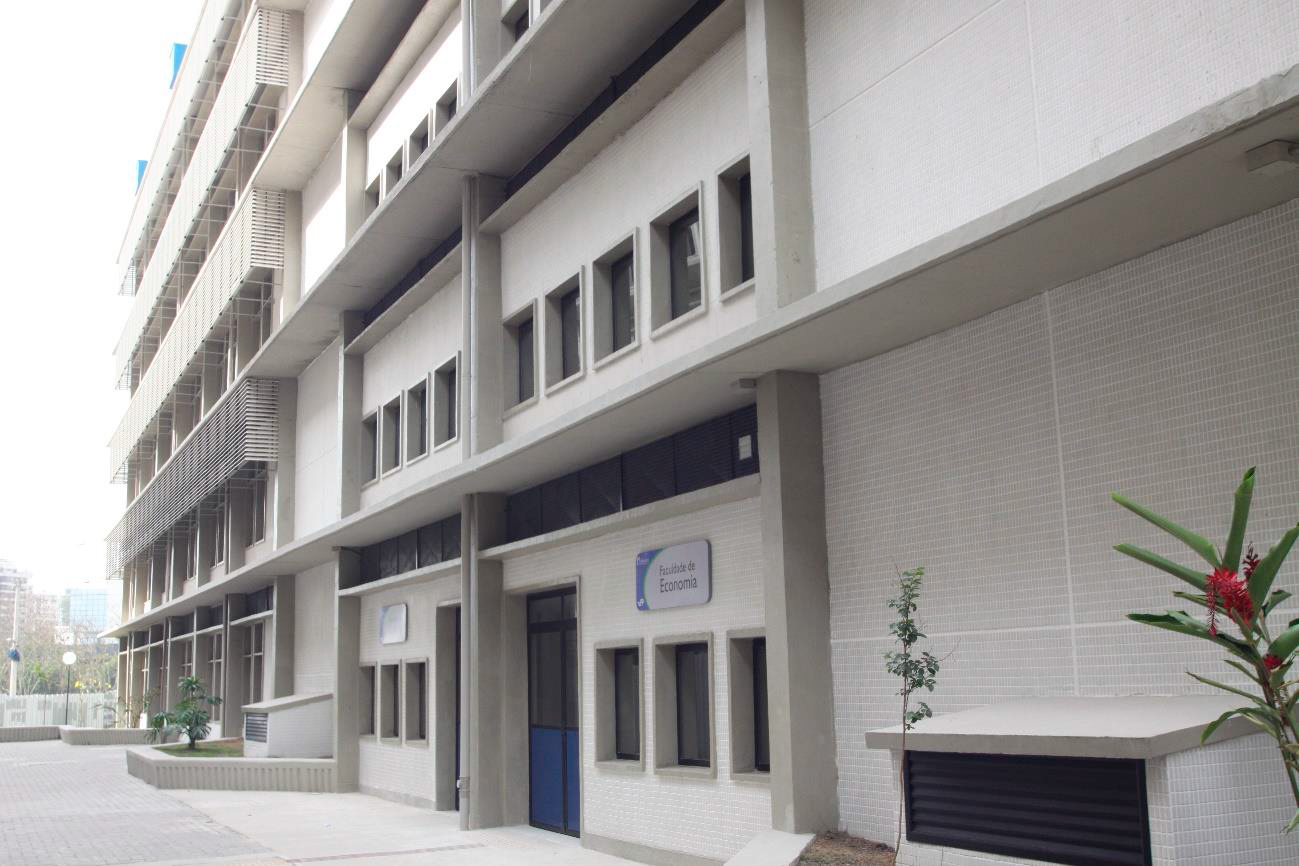
\includegraphics[width=\textwidth]{ecouff.jpg}
\caption{Exemplo de Imagem}
\end{figure}

%---------------------------------------------------------
% seção exemplo de ambiente matematico
%---------------------------------------------------------

\section{Ambiente Matemático}

Se quero escrever algo num ambiente matemático, escrevo normalmente:

$$f(x)=\frac{1}{\sqrt{2\pi\sigma^2}}exp\left[\frac{-1}{2}\left(\frac{x-\mu}{\sigma}\right)\right]$$\\

A próxima seção é um exemplo de referência bibliográfica. Este documento tenta manter um padrão parecido ao ABNT, levando em consideração fonte, margem, formato de citação e referência bibliográfica.

\nocite{frisch2009problems}

\bibliography{refs}


\end{document}
